%!TEX root = ../main.tex
\doublespacing
\chapter{Theoretical Background}
\label{chap:theory}
The following chapter describes the main theoretical concepts relevant to this thesis. In order to understand the corona, one must understand the plasma it is made of. Thus, I start in section \ref{sec:plasma_intro} with some fundamental concepts of plasma physics and introduce the kinetic theory of plasmas by considering the distribution of many particles in a six dimensional phase space. This lays the groundwork for a fluid description of plasmas, magnetohydrodynamics (MHD), arguably the most useful description of a plasma in the context of the solar corona which is discussed in section \ref{sec:MHD}. The MHD equations are investigated further to determine how longitudinal and transverse waves propagate in a plasma which is relevant for the subsequent discussion of Langmuir wave generation and the plasma emission mechanism of type III radio bursts in section \ref{sec:plasma_emission}. Section \ref{sec:scattering_theory} gives an overview of the theory of radio wave scattering in the corona and concludes this chapter. 
% and a discussion about the power spectrum of electron density fluctuations in section \ref{sec:density_fluctuations} concludes this chapter.


\section{Introductory Concepts in Plasma Physics}
\label{sec:plasma_intro}
Plasma was the name given by Langmuir to the new, exotic type of matter he was studying in the 1920s. It is essentially an ionized gas that exhibits quasi-neutrality on a macroscopic scale. The solar corona is a shell of hot plasma surrounding the Sun and as such, the study of emission from the corona is a study of the plasma itself. A plasma's tendency to remain in quasi-neutrality means that any change to the charge separation between electrons and ions generates an electric field which acts as a restoring force and thus oscillations are induced in the plasma. To determine the frequency of these oscillations imagine the following, a plasma with equal number density of electrons and ions $N_e = N_i = N_0$ is perturbed so that a group of electrons are moved by some distance $x$ a restoring force $\mathbf{E} = q_e E_x$ acts to bring the electrons back to their initial position. Due to their mass, the electrons overshoot their initial position and the process begins again in the opposite direction. Here we have made the safe assumption that, due to electrons being much lighter, the ions remain stationary. For electrons with mass $m_e$, Newton's second law gives us,
\begin{equation}
\label{eq:fma}
m_e \frac{d^2x}{dt^2} = q_e E_x.
\end{equation}
Gauss' law for some closed, rectangular box surface, $S$, inside our perturbed plasma gives, 
$$
\oint_S \mathbf{E} \cdot d\mathbf{s} = \frac{Q}{\epsilon_0}
$$
where $Q$ is the total charge contained within the closed surface $S$. Given the equilibrium density of electrons, $N_e$, the total charge must be $Q = A x N_e q_e$ where $A$ is the cross-sectional area of $S$. For $A=a\Delta z$, we can solve for  $E_x$ to find,
$$
\oint_S \mathbf{E} \cdot d\mathbf{s} = -a \Delta z E_x =  \frac{Q}{\epsilon_0} = \frac{ax\Delta z N_e q_e}{\epsilon_0} \rightarrow E_x = -\frac{x N_e q_e}{\epsilon_0}.
$$
Using this with Equation \ref{eq:fma} we obtain the ordinary differential equation,
\begin{equation}
\label{plasma_motion}
m_e \frac{d^2 x}{dt^2} + \frac{N_e q_e^2}{\epsilon_0} x = 0 \rightarrow \frac{d^2 x}{dt^2} + \omega_p^2 x = 0.
\end{equation}
The solution to this equation is the well known harmonic oscillator with an angular frequency $\omega_p$ which we call the electron plasma frequency or simply, the plasma frequency
\begin{equation}
\label{eq:plasma_freq}
\omega_p = \sqrt{\frac{N_e q_e^2}{\epsilon_0 m_e}}.
\end{equation}
The plasma frequency leads us to an important criterion that a partially ionised gas must have to be considered a plasma. That is, plasma oscillations can only develop if the mean free time between collisions of electrons and ions with neutrals, $\tau_n$, is longer than the oscillation period $\tau_p = 1/ \omega_p$, or $\omega_p \tau_n >1$.

Another implication of the quasi-neutrality of plasmas can be seen when one considers immersing a test particle of charge $Q_+$ inside an initially uniform plasma at time $t = 0$ such that, again, $N_i = N_e = N_0$. The electric potential in the plasma is that due to the single test charge, 
$$
\Phi (\mathbf{r}) = \frac{1}{4 \pi \epsilon_0} \frac{Q}{r},
$$
assuming the test charge is at the origin of our spherical coordinate system. Once again we assume that because the ions are much more massive compared to the electrons in the plasma that their motion can be neglected. The electrons in the plasma are attracted to the test charge causing the electron density near the test charge to increase. The new potential distribution $\Phi (\mathbf{r})$ must be re-evaluated using Poisson's equation:
\begin{equation}
\label{eq:test_charge}
\nabla^2 \Phi (\mathbf{r}) = - \frac{\rho}{\epsilon_0} = - \frac{q_e(N_e - N_i)}{\epsilon_0},
\end{equation}
where the excess free charge density near the test charge is $\rho = q_e (N_e - N_i)$. In spherical coordinates this leads to an electron density distribution of,
\begin{equation}
\label{eq:e_density}
N_e(r) = N_0 e^{-q_e \Phi (r)/k_b T_e}
\end{equation}
where $k_B$ is Boltzman's constant and $T_e$ is the electron temperature. Subbing into the spherical coordinate version of Equation \ref{eq:test_charge} gives,
\begin{equation}
\label{eq:spherical_poisson}
\frac{1}{r^2} \frac{d}{dr}\left(r^2 \frac{d \Phi}{dr} \right) = - \frac{q_e N_0}{\epsilon_0}\left[\exp\left(\frac{-q_e \Phi (r)}{k_BT}\right) -1 \right],\  r>0.
\end{equation}
Assuming $\vert q_e \Phi \vert \ll k_b T$, Equation \ref{eq:spherical_poisson} can be expanded as a power series to give, 
$$
\frac{1}{r^2} \frac{d}{dr}\left(r^2 \frac{d \Phi}{dr} \right) \simeq \left[ \frac{N_0q_e^2}{\epsilon_0 k_B T_e} \right]\Phi (r) = \frac{1}{\lambda_D^2}\Phi(r)
$$
where $\lambda_D$, known as the Debye length, is defined to be
\begin{equation}
\label{eq:debye_length}
\lambda_D = \sqrt{\frac{\epsilon_0 k_B T_e}{N_0 q_e^2}}.
\end{equation}
The solution to the above can be found to be 
\begin{equation}
\label{eq:phi_solution}
\Phi (r) = \left[ \frac{1}{4 \pi \epsilon_0} \frac{Q}{r}\right] e^{-r/\lambda_D},
\end{equation} 
which shows that for $r \gg \lambda_D$, the potential of the test charge disappears. Thus the Debye length of a plasma can be used to define a second plasma criterion: an ionised gas can only be considered a plasma if the length scale of the system, $L$, is much greater than the Debye length.
\subsection{Kinetic Theory}
Armed with some knowledge of fundamental plasma behaviour, we jump forward through plasma theory to determine the collective properties of plasmas using averages over large numbers of particles. In order to do so, the positions and velocities of plasma particles are described using a distribution function in an approach called plasma kinetic theory. For now the exact form of this distribution function does not matter. We start by assuming that the position of each particle in our plasma is given by a vector $\mathbf{r}$ from the origin where,
\begin{equation}
\label{eq:KT_position}
\mathbf{r} = \mathbf{\hat{x}}x + \mathbf{\hat{y}}y + \mathbf{\hat{z}}z
\end{equation}
and that each particle has a linear velocity,
\begin{equation}
\label{eq:KT_velocity}
\mathbf{v} = \mathbf{\hat{x}}v_x + \mathbf{\hat{y}}v_y + \mathbf{\hat{z}}v_z
\end{equation}
so that the particle speed is $\vert \mathbf{v} \vert = v = \sqrt{v_x^2 + v_y^2 + v_z^2}$. Thus, at any given time, the position and velocity of a particle can be represented as a point in a six dimensional phase space determined by the coordinates $x, y, z, v_x, v_y$ and $v_z$. Now consider a volume element $d\mathbf{r} = d^3r = dxdydz$ such that it is large enough to contain a great number of particles but small enough so that macroscopic quantities vary only slightly inside it. Also consider a time interval $dt$ centred around time $t$, where $dt$ is long compared to the mean time for a particle to traverse $d\mathbf{r}$ but similarly short enough compared to the time scales of the macroscopic parameters of the plasma. The number of particles in $d\mathbf{r}$ averaged over $dt$ is simply $N(\mathbf{r},t)d\mathbf{r}$ where $N(\mathbf{r},t)$ is the number density of particles. In the same manner, one can define a density of the number of particles in velocity space which we denote as $f(\mathbf{r}, \mathbf{v}, t)d\mathbf{r}$. From this, we can determine the number of particles at time $t$ in the element $d\mathbf{r}$ and with velocities between $\mathbf{v}$ and $\mathbf{v} + d\mathbf{v}$ is $f(\mathbf{r}, \mathbf{v}, t)d\mathbf{r}d\mathbf{v}$ The function $f(\mathbf{r}, \mathbf{v}, t)$ is called the velocity distribution function and is the density of representative points in phase space. The total number of velocity points in all of velocity space can be found by summing the number of velocity points $f(\mathbf{r}, \mathbf{v}, t)d\mathbf{r}d\mathbf{v}$ in $d\mathbf{v}$ over all possible velocities. Following from this, we can obtain the number density of particles:
\begin{equation}
\label{eq:KT_number_density}
N(\mathbf{r},t) =\int^\infty_{-\infty}  f(\mathbf{r}, \mathbf{v}, t) d\mathbf{v}.
\end{equation}

Other macroscopic plasma parameters (e.g. mass density, flux, current) can be obtained using the velocity distribution function. Consider any property $g(\mathbf{r},\mathbf{v}, t)$ of a particle. The average value of this quantity is given by
\begin{equation}
\label{eq:KT_average_value}
g_{\mbox{av}}(\mathbf{r}, t)  = \langle g(\mathbf{r}, \mathbf{v}, t) \rangle = \frac{1}{N(\mathbf{r}, t)} \int g(\mathbf{r}, \mathbf{v}, t) f(\mathbf{r}, \mathbf{v}, t) d\mathbf{v}.
\end{equation}
The evolution of the velocity distribution function, which we henceforth refer to as the distribution function, or $f$, in time is determined by the Boltzmann Equation:
\begin{equation}
\label{eq:KT_Boltzmann_eq}
\frac{\partial f}{\partial t} + (\mathbf{v} \cdot \nabla_\mathbf{r})f + \left[ \left(\frac{\mathbf{F}}{m} \right) \cdot \nabla_\mathbf{v}\right]f = \left( \frac{\partial f}{\partial t} \right)_{\mbox{coll}}
\end{equation}
where $\mathbf{F} =m\mathbf{a}$ is a force acting on the particles.
The Boltzmann equation is essentially a statement on the conservation of points in phase space. The left hand side describes particle flow through the volume element $d\mathbf{r} d\mathbf{v}$ and it is balanced by the collisional term on the right hand side. By considering a homogeneous plasma in a steady-state (i.e. in thermal equilibrium) with no external forces, the terms on the left hand side of the Boltzmann equation all become 0 and thus 
$$
\left( \frac{\partial f}{\partial t} \right)_{\mbox{coll}} = 0.
$$
By considering the particle collisions in which energy must be conserved under the above assumptions it can be shown that the distribution function takes the form of the Maxwell-Boltzmann distribution:
\begin{equation}
\label{eq:KT_maxwellboltzmann}
f(\mathbf{r}, \mathbf{v}, t) = f(v) = N_0 \left( \frac{m}{2 \pi k_B T} \right)^{\frac{3}{2}} e^{-mv^2/(2K_BT)}.
\end{equation}
By substituting the Lorentz force into \ref{eq:KT_Boltzmann_eq}, assuming no collisions, gives the Vlasov equation:
\begin{equation}
\label{eq:KT_Vlasov_eq}
\frac{\partial f}{\partial t} + (\mathbf{v} \cdot \nabla_\mathbf{r})f + \frac{q}{m} \left[ \left(\mathbf{E} + \mathbf{v} \times \mathbf{B} \right) \cdot \nabla_\mathbf{v}\right]f = 0. 
\end{equation}
The Vlasov equation, together with Maxwell's equations for $\mathbf{E}$ and $\mathbf{B}$ represent a complete set of self-consistent equations to describe a plasma interacting with an electromagnetical field. So far we have considered the derivatives of $f$ with respect to a stationary reference frame. It is more convenient to consider a reference frame that moves with the fluid elements of a plasma. A derivative in this sense is known as a convective derivative or total time derivative and can be expressed for the distribution function as
\begin{equation}
\label{eq:KT_Vlasov_convective}
\frac{df}{dt} = \frac{\partial f}{\partial t} + (\mathbf{v} \cdot \nabla_\mathbf{r})f + \left(\frac{d\mathbf{v}}{dt} \cdot \nabla_\mathbf{v}\right)f.
\end{equation}
Thich has the interesting result that the collisionless Boltzmann equation can be written as
\begin{equation}
\label{eq:KT_Liouville}
\frac{df}{dt}=0,
\end{equation}
meaning that a particle moving through phase space will see a constant $f$ in its local frame. This is known as Liouville's theorem. The Boltzmann equation allows us to determine the macroscopic transport equations of a plasma, which will form the foundations of the theory in the section to come. This is done not by solving the Boltzmann equation itself but rather, multiplying it by various powers of $\mathbf{v}$ and integrating over velocity, i.e. ``taking the moments of the Boltzmann equation"
$$
\mu_n = \int \mathbf{v}^n\left[\mbox{Boltzmann Eq.}\right]dv,
$$
where $\mu_n$ is the $n$th order moment. This procedure gives up our knowledge on the velocity distribution of particles in order to instead obtain single-value macroscopic particles of a plasma fluid. The main results for the first 3 moments are shown here \footnote{The interested reader is referred to e.g. \cite{Inan2010} for a full derivation of these equations.}:
\begin{align*}
& \mu_0 \rightarrow  \mbox{continuity equation or conservation of mass} \\
& \mu_1 \rightarrow  \mbox{momentum transport equation or conservation of momentum} \\
& \mu_2 \rightarrow  \mbox{energy transport equation or conservation of energy}
\end{align*}
The moments of the Boltzmann equation allows us to develop the theory of plasmas as being made up of multiple fluids each of their different particle species, e.g. electrons and ions. Under certain conditions it is possible to consider the entire plasma as a single fluid and it is this approach, called magnetohydrodynamics, that I discuss next\footnote{The derivations of the equations of motion for a two-fluid plasma and their subsequent combination to a single fluid are complex and tedious. I therefore once again refer an interested reader to e.g. \cite{Inan2010}}.
\section{Magnetohydrodynamics}
\label{sec:MHD}
Magnetohydrodynamics (MHD) is a framework to describe the dynamics of an electrically conducting fluid in the presence of a magnetic field. It is a useful method that can be used to model large-scale, slowly varying plasma phenomena in a highly ionised plasma. For plasmas that are either collision-dominated or contain a strong external magnetic field the MHD description of a plasma is particularly appropriate. Given that these conditions are met in the solar corona, it is worth expanding upon some key ideas of MHD theory. For now we assume a collison-dominated plasma but the same ideas can be applied to collisionless plasmas with strong magnetic fields.

The single fluid equations, derived from the moments of the Boltzmann equation, and the generalised Ohm's law can be simplified using several approximations to form what are known as the simplified MHD equations.
\begin{subequations} \label{eq:MHD_simplified}
\begin{align}
\mathbf{J} = \sigma(\mathbf{E} + \mathbf{u}_m \times \mathbf{B}) \\
\frac{\partial \rho_m}{\partial t} + \rho_{m0} \nabla \cdot \mathbf{u}_m = 0 \\
\rho_m \frac{\partial \mathbf{u}_m}{\partial t} = - \nabla p + \mathbf{J} \times \mathbf{B}
\end{align}
\end{subequations}
where $\mathbf{J}$ is the current density, $\sigma$ is the electrical conductivity, $\rho_m$ is the (variable) mass density, $\rho_{m0}$ is the (relatively constant) mass density,  $\mathbf{u}_m$ is the mass velocity and $p$ is the pressure.
The electromagnetic fields inside a plasma are governed by Maxwell's equations,
\begin{subequations} \label{eq:MHD_Maxwell}
\begin{align}
& \nabla \cdot \mathbf{E} = \frac{\rho}{\epsilon_0} = 0 \\
& \nabla \cdot \mathbf{B} = 0 \\
& \nabla \times \mathbf{E} = - \frac{\partial \mathbf{B}}{\partial t} \\
& \nabla \times \mathbf{B} = \mu_0 \mathbf{J}
\end{align}
\end{subequations}
where the assumption of no accumulation of charge inside the fluid gives rise to the charge density $\rho = 0$. Finally, by assuming an adiabatic equation of state,
\begin{equation}
\label{eq:MHD_eq_of_state}
\frac{d}{dt} \left(p \rho_m^{-\gamma} \right) = 0
\end{equation}
where $\gamma $ is the adiabatic index.
Equations \ref{eq:MHD_simplified}, \ref{eq:MHD_Maxwell} and \ref{eq:MHD_eq_of_state} form a closed system which can be solved for any of the fluid or electromagnetic variables. These equations can be used to describe some simple wave phenomena that MHD plasmas exhibit which are relevant to the later discussion of the plasma emission mechanism.
\subsection{Waves in Plasmas}
As we shall see shortly, the generation and propagation of waves in plasmas can result in the emission of electromagnetic radiation which, in turn, must travel through the plasma. Consequently, it is important to outline the basics of waves in plasmas. In the following we only consider waves of small amplitude superimposed on a background of a uniform, unmagnetised plasma. Background quantities will be denoted by a subsrcipt of `0', while the perturbed quantities will be given a  subscript `1'. We also only consider the case where there is no steady fluid motion and no external electric field. Thus we can write the simplified MHD equations (assuming no collisions and an adiabatic equation of state) as
\begin{subequations} \label{eq:MHDwaves_simplified}
\begin{align}
& \frac{\partial N_1}{\partial t} + N_0 \nabla \cdot \mathbf{u} = 0 \\
& N_0 m \frac{\partial \mathbf{u}}{\partial t} = q N_0 (\mathbf{E} + \mathbf{u} \times \mathbf{B}_0) - \nabla p_1 \\
& \frac{p_1}{p_0} = \gamma \frac{N_1}{N_0} \rightarrow p_1 = \gamma k_B T N_1 
\end{align}
\end{subequations}
where the assumption that each particle species is an isothermal gas with temperature $T$ gives $p_0 = N_0 k_b T$. Maxwell's equations then become
\begin{subequations} \label{eq:MHDwaves_Maxwell}
\begin{align}
& \nabla \cdot \mathbf{E} = \frac{\rho_1}{\epsilon_0} \\
& \nabla \cdot \mathbf{B}_1 = 0 \\
& \nabla \times \mathbf{E} = - \frac{\partial \mathbf{B}_1}{\partial t} \\
& \nabla \times \mathbf{B}_1 = \mu_0 \mathbf{J} + \epsilon_0 \frac{\partial \mathbf{E}}{\partial t}
\end{align}
\end{subequations}
In order to study plane waves, solutions of the above where all perturbation quantities vary proportionally to  $e^{i(\omega t - \mathbf{k} \cdot \mathbf{r})}$ are sought. In the following we use the fact that for solutions of this form $\partial / \partial t \rightarrow i \omega$ and $\nabla \rightarrow -i \mathbf{k}$.  For a cold plasma with $T=0$ the equation of motion of the electrons is reduced to 
\begin{equation}
\label{eq:MHDwave_clodplasma}
m_e i \omega \mathbf{u}_e = q_e \mathbf{E}
\end{equation}
Taking the divergence of \ref{eq:MHDwave_clodplasma} and using \ref{eq:MHDwaves_simplified}a gives
\begin{equation}
N_1 = \frac{N_0 q_e}{m_e \omega^2} \nabla \cdot \mathbf{E} \rightarrow \rho_1 = N_1 q_e - \frac{N_0 q_e^2}{m_e \omega^2} \nabla \cdot \mathbf{E}.
\end{equation}
For a longitudinal wave $\nabla \cdot \mathbf{E} \neq 0$ and thus, using \ref{eq:MHDwaves_Maxwell}a, we must have
\begin{equation}
\label{eq:MHDwave_plasmafreq}
\omega^2 = \frac{N_0 q_e^2}{m_e \epsilon_0} \equiv \omega^2_{p}
\end{equation}
which is the plasma frequency we found earlier from our discussion at the beginning of Section\ref{sec:plasma_intro}! Note also that, because $\omega$ does not depend on $\mathbf{k}$, the group velocity $v_g = d\omega / d k$ of this wave is 0. This means that the plasma oscillation does not propagate from the location where they are generated. For a magnetised plasma with finite temperature the dispersion relation of Langmuir waves becomes 
\begin{equation}
\label{eq:MHDwave_langmuir}
\omega^2 = \omega_p^2(1 + \gamma \lambda_D^2k^2).
\end{equation}
This propagating plasma oscillation is known as a Langmuir wave and will be instrumental in describing the process of plasma emission in a type III radio burst.

Electromagnetic waves traveling through a plasma have their own dispersion relation which can be found from the refractive index
\begin{equation}
\mu \equiv \frac{kc}{\omega} = (1 - \frac{\omega_p^2}{\omega^2})^{\frac{1}{2}}
\end{equation}
to be
\begin{equation}
\label{eq:MHDwave_emdispersion}
\omega = (\omega_p +k^2 c^2)^\frac{1}{2}.
\end{equation}
Here it is obvious that $\omega_p$ acts as a cutoff frequency, below which electromagnetic waves become evanescent and are rapidly attenuated.
\section{The Plasma Emission Mechanism}
\label{sec:plasma_emission}
The plasma emission mechanism occurs over a number of stages. First, an instability must be generated in the velocity distribution function. This leads to the growth of Langmuir waves before finally these Langmuir waves are converted to transverse electromagnetic waves. In a type III radio burst a high velocity, low density, electron beam passes through the background plasma to form a ``bump on tail" distribution. This distribution is unstable and leads to the growth of Langmuir waves. These Langmuir waves in turn generate electromagnetic waves by coalescing with other Langmuir waves or by decaying. The electromagnetic waves are the radio bursts that are observed. In this section the generation of Langmuir waves in 1D and the process of plasma emission are discussed under the framework of quasi-linear theory.

\begin{figure}[ht]
\centering
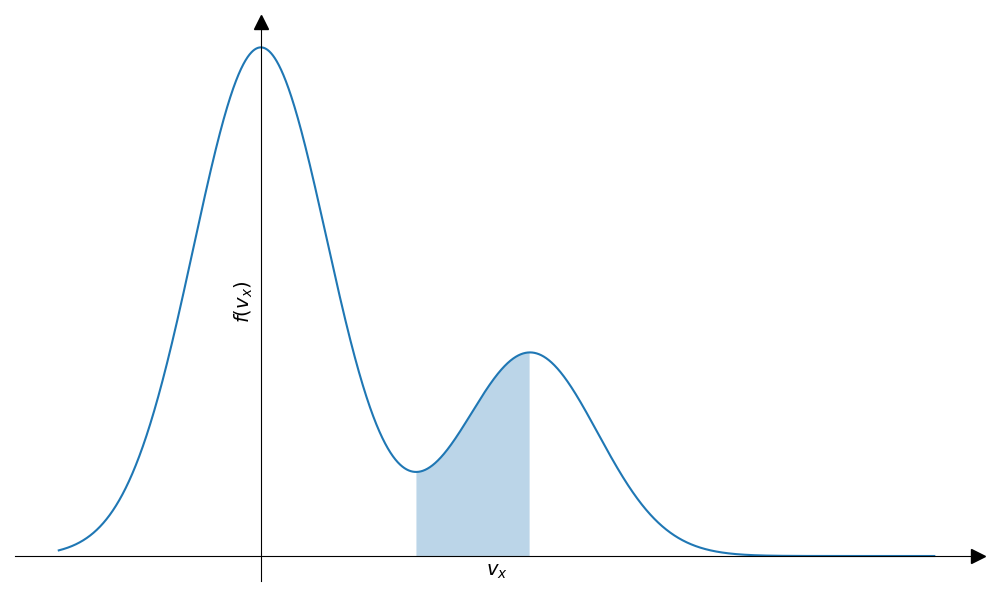
\includegraphics[width=0.75\columnwidth]{Bump_on_tail.png}
\caption[A ``bump on tail" distribution.]{The 1D electron velocity distribution function of a background plasma and a low density, high velocity electron beam. This is known as the ``bump on tail" distribution. The shaded region indicates where the gradient of the distribution function is positive and can excite Langmuir waves in the background plasma.}
\label{fig:bumpontail}
\end{figure}

\subsection{Generation of Langmuir Waves}
During magnetic reconnection electrons can be accelerated along magnetic field lines. As these beams of electrons propagate, faster electrons begin to outpace slower electrons and stationary ions in the background plasma. This leads to a second peak on the Maxwell-Boltzmann distribution of velocities as seen in Figure \ref{fig:bumpontail}. Energy is transferred from electrons travelling at the phase velocity, $v_{\phi}$ , to Langmuir waves creating a resonance.
The positive velocity gradient of this resonance means that there are more electrons with velocity greater than $v_{\phi}$ than there are electrons with velocities less than  $v_{\phi}$ (where energy is transferred from the wave to the particles), this causes Langmuir waves to become unstable and their magnitudes to grow exponentially. Particles with velocities near $v_{\phi}$ are in resonance with the Langmuir waves and drive this instability.

In the following, the electron velocity distribution function is described as the sum of a slowly varying part $f_0$ and a rapidly oscillating part $f_1$, where $\vert f_1 \vert \ll f_0$
\begin{equation}
\label{eq:ql_distributionf}
f(\mathbf{r}, \mathbf{v}, t) = f_0(\mathbf{v}) + f_1(\mathbf{r}, \mathbf{v}, t).
\end{equation} 
Equation \ref{eq:ql_distributionf} can now be substituted into the Vlasov Equation (Equation \ref{eq:KT_Vlasov_eq}), where we note that $\mathbf{E}$ and $f_1$ are perturbation quantities. By neglecting second order terms and assuming an unmagnetised plasma, i.e. $\mathbf{B} = 0$, we obtain the linearalised Vlasov Equation
\begin{equation}
\label{eq:linear_vlasov}
\frac{\partial f_1}{\partial t} + (\mathbf{v} \cdot \nabla)f_1 + \frac{q_e}{m_e} \mathbf{E} \cdot \nabla_\mathbf{v}f_0 = 0.
\end{equation} 
It can be shown that in 1D the electron distribution function, $f(v,t)$ where $\int f(v,t) dv = n_e$, and the spectral energy density of Langmuir waves, $W(v,t)$ such that $\int W(v,t) dv = E_L$ the total energy density, can be expressed as follows \citep{Vedenov1963,Reid2014},
\begin{equation}\label{eq:dfdt}
    \frac{\partial f(v,t)}{\partial t}=\frac{4 \pi^2 e^2}{m_e^2} \frac{\partial}{\partial v} \left( \frac{W}{v} \right) \frac{\partial f(v,t)}{\partial v}
\end{equation}

\begin{equation}\label{eq:dWdt}
    \frac{\partial W(v,t)}{\partial t}= \frac{\pi \omega_p}{n_e} v^2 W \frac{\partial f(v,t)}{\partial v}
\end{equation}

Equation \ref{eq:dWdt} shows that the growth rate of Langmuir waves is proportional to $\frac{\partial f(v,t)}{\partial v}$, hence a positive gradient in the Maxwell Boltzmann distribution leads to a growth in Langmuir waves. The right hand side of Eq. \ref{eq:dfdt} has a diffusion operator $D=\frac{W}{v}$. This states that the transfer of energy from particles to waves and back leads to the distribution function being smoothed out and eventually becoming a plateau. The evolution of $f(v,t)$ and $W(v,t)$ with time is shown in Figure \ref{fig:Lwavegrowth}.  As time progresses, a plateau is formed in the distribution function and a broadening of the spectral energy density develops.	 This process is known as quasi-linear relaxation \citep{Melrose1987}.
%The instability is alleviated by what is known as quasi-linear relaxation \citep{Melrose1987} whereby the resonant behaviour of the electrons and Langmuir waves results in a plateau in the Maxwell Boltzmann distribution rather than a second peak. Figure \ref{fig:Lwavegrowth} shows the evolution of the velocity distribution fucntion (left) and spectral energy density of Langmuir waves (right) with time. 
\begin{figure}[ht]
    \centering
    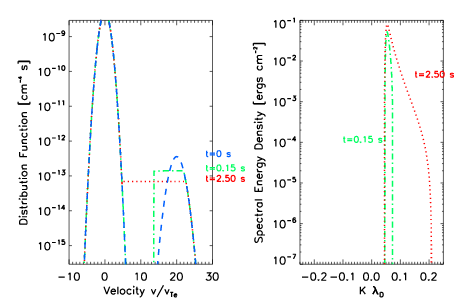
\includegraphics[width=\columnwidth]{Images/L_wave_growth.png}
    \caption[Langmuir wave distriburtion function and spectral energy density.]{Left: Evolution of distribution function (normalised by the electron thermal velocity $v_{Te}=V_e$) in time. The diffusive term in \ref{eq:dfdt} causes the bump-on-tail Gaussian to turn into a plateau, thereby eliminating the instability caused by the positive velocity gradient. Right: The spectral energy density of generated Langmuir waves, x-axis normalised to the Debye length $\lambda_D=\sqrt{\frac{\epsilon_0 k_B T_e}{e^2 n_e}}$. Each panel shows successive times of t=0.15s (green, dot-dashed line) and t=2.50s (red, dotted line). Figure taken from \cite{Reid2014}.} %(Figure taken from \citeauthor{Reid2014} \citeyear{Reid2014})}
    \label{fig:Lwavegrowth}
\end{figure}

\subsection{Wave-Wave Interaction}\label{Plasma Emission}
Now that we know how Langmuir waves are generated by an unstable distribution, we must discuss how these Langmuir waves are converted to electromagnetic waves via wave-wave interactions. Wave-wave interaction concerns the processes by which three types of waves interact. These are: transverse (T) waves, Langmuir (L) waves and ion sound (S) waves, and have the following, respective, dispersion relations:
$$ \omega_T=(\omega_p^2 +k^2c^2)^{\frac{1}{2}} $$
$$ \omega_L \cong \omega_p + \frac{3k^2V_e^2}{2 \omega_p}$$
$$ \omega_S = kv_s $$
where $V_e$ is the thermal velocity of electrons in the plasma, $v_s$ is the ion sound speed and $k$ is the wave vector. Only transverse waves with $\omega > \omega_p $ can escape and thus a plasma emission mechanism is a process that generates these transverse waves. 

As mentioned in Section \ref{sec:typeIII}, type III bursts have a harmonic structure associated with plasma emission at the plasma frequency and the second harmonic. Both of these transverse waves are formed in different three wave processes that will now be discussed.
In a plasma, due to scattering from other wave modes and ions in the plasma, a wave mode can be changed from one to the other \citep{McLean1985, Melrose1987}. This is expressed in the equation 
$$ \sigma \rightleftarrows \sigma' + \sigma '' $$
where $\sigma$, $\sigma'$  and  $\sigma ''$ represent different wave modes. Conservation of energy and momentum state \citep{McLean1985},
$$ \omega^{\sigma}(k)=\omega^{\sigma'}(k')+\omega^{\sigma''}(k'')$$
$$ k=k'+k''$$
where $ \omega^{\sigma}(k)$ is the frequency of a particular wave mode with the wave vector $k$. For Langmuir (L), ion sound (S) and transverse (T) wave modes the allowed processes are \citep{Melrose1987}:
\begin{align*}
& L+S \rightarrow L^\prime \\
& L+S \rightarrow T \\
& L \rightarrow T + S \\
& L \rightarrow L^\prime + S \\
& T+S \rightarrow L \\
& T+S\rightarrow T^\prime \\ 
& L+L^\prime \rightarrow T.
\end{align*}
Of these L+S$\rightarrow$T and L$\rightarrow$T+S are responsible for fundamental emission while harmonic emission is associated with the three wave process L+L$^\prime \rightarrow$T \citep{Melrose1987}.

Originally \cite{Ginzburg1958} considered fundamental emission to be due to Langmuir waves scattering off of thermal ions in the plasma. It is now commonly accepted that the biggest cause of fundamental emission is due to the three wave processes of a Langmuir wave coalescing with an ion sound wave generated by L$\rightarrow$L$^\prime$+S or when a Langmuir wave decays into an ion sound wave and an electromagnetic transverse wave. The process L$\rightarrow$T+S can be visualised as in Figure \ref{fig:Femission}. In solar radio physics it is often assumed that $k_L \gg k_T$, knowing this and that the wave vectors must satisfy $\mathbf{k}_L \pm \mathbf{k}_s = \mathbf{k}_T$ ($+$ for L+S$\rightarrow$T , $-$ for L$\rightarrow$T+S) implies $\mathbf{k}_s \approx \mp \mathbf{k}_L$.

\begin{figure}[ht]
\centering
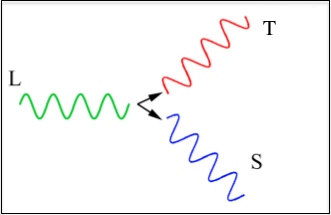
\includegraphics[width=0.5\columnwidth]{Images/Fundamental_emission_Lwaves.png}
\caption[A three wave process of fundamental plasma emission L$\rightarrow$T+S.]{A three wave process of fundamental plasma emission L$\rightarrow$T+S. A Langmuir wave decaying into an ion sound wave and an electromagnetic transverse wave at the plasma frequency. (Figure adapted from Solar (interplanetary) Radio Bursts: the Generation of Radio Waves,	an oral presentation by David Malaspina at the Jean Louis Steinberg International Workshop on Solar, Heliospheric and Magnetospheric Radioastronomy, November 2017)}
\label{fig:Femission}
\end{figure}

Second harmonic emission occurs when two Langmuir waves coalesce in the process L+L$^\prime \rightarrow$T, shown in Figure \ref{fig:Hemission}. Conservation of momentum requires that $\mathbf{k}_L + \mathbf{k'}_L = \mathbf{k}_T$ and for second harmonic (H) generation, $k_T=k_H \approx \frac{\sqrt{3} \omega_p}{c}$. The phase speed $v_\phi$ of Langmuir waves is much less than $\frac{c}{\sqrt{3}}$ meaning that $k_L \gg k_T$ which results in $\mathbf{k}_L \approx -\mathbf{k'}_L$. This means that for a transverse wave at the second harmonic to be created, two Langmuir waves must coalesce almost exactly head on. These backward propagating Langmuir waves are generated: in the three wave processes of L+S$\rightarrow$L$^\prime$ and L$\rightarrow$L$^\prime$+S, i.e. scattering off of thermal ions, and by refraction at density inhomogeneities.
 \begin{figure}[ht]

     \centering
     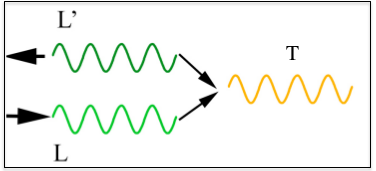
\includegraphics[width=0.5\columnwidth]{Images/Harmonic_emission_Lwaves.png}
     \caption[Three wave process of second harmonic plasma emission L+L' $\rightarrow$ T.]{Three wave process of second harmonic plasma emission L+L' $\rightarrow$ T. A Langmuir wave (L) and a backwards propagating Langmuir wave (L') coalesce to form a transverse wave (T) at $2 \omega_p$. (Figure adapted from Solar (interplanetary) Radio Bursts: the Generation of Radio Waves,	an oral presentation by David Malaspina at the Jean Louis Steinberg International Workshop on Solar, Heliospheric and Magnetospheric Radioastronomy, November 2017)}
     \label{fig:Hemission}
 \end{figure}
 
\section{Scattering of radio wave light in the solar corona}
\label{sec:scattering_theory}

\cite{Chandrasekhar1952} outlined a statistical description of ``stellar scintillation" in order to account for observations with astronomical seeing.  The basis of this description is that a plane wave front travels through a turbulent layer whose refractive index, $\mu$, is subject to random fluctuations. The auto correlation function of these fluctuations at two different points $\mathbf{r_1}$ and $\mathbf{r_2}$ is given by
$$
\frac{\langle \delta \mu(\mathbf{r_1}) \delta \mu(\mathbf{r_2}) \rangle}{\langle \delta^2 \mu \rangle}, 
$$
and can be defined to be some function $M(r)$ only of the distance between the two points $r = \vert \mathbf{r_1} - \mathbf{r_2} \vert$. For the remainder of this section I will describe the \cite{Chandrasekhar1952} treatment of scintillations for a ``disturbed layer" in the atmosphere and how this was adopted by \cite{Fokker1965}, \cite{Steinberg1971} and \cite{Riddle1974} to explain observed characteristics of radio bursts before finally discussing the modern approach to radio wave scattering.

Under the assumptions of homogeneity and isotropy, the correlation between refractive index fluctuations in the layer will depend only on distance between two points. Thus
\begin{equation}
\label{eq:scattering_correlation}
\langle \delta \mu(\mathbf{r_1}) \delta \mu(\mathbf{r_2}) \rangle = \langle \delta^2 \mu \rangle M(r),
\end{equation}
where $\langle \delta^2 \mu \rangle$ is the mean squared fluctuation of refractive index and $M(r)$ is some (even) function of $r$. 
%For reasons that will become apparent, we introduce the tensor
%\begin{equation}
%\label{eq:scattering_tensor}
%R_{ij} = \bigg \langle \left( \frac{\partial}{\partial x_i} \delta \mu \right) \left( \frac{\partial}{\partial {x_j}' } \delta \mu \right) \bigg \rangle
%\end{equation}
%which gives the correlation of a component $\nabla \delta \mu$ at a point $x_i$ with that at a point ${x_i}'$. For $\xi_i = {x_i}' - x_i$ the tensor becomes
%\begin{equation}
%\label{eq:scattering_tensor2}
%R_{ij} = - \langle \delta^2 \mu \rangle \frac{\partial^2 M}{\partial \xi_i \partial \xi_j} = - \langle \delta^2 \mu \rangle \left[\left(\frac{M^{\prime\prime}}{r^2} - \frac{M^ \prime}{r^3}\right) \xi_i \xi_j + \frac{M^\prime}{r}\delta_{ij}\right],
%\end{equation} 
%where primes denote differentiation with respect to $r$.  In particular we can show that
%\begin{equation}
%\label{eq:scattering_transverse_correlation}
%\bigg \langle \left( \frac{\partial}{\partial x_i} \delta \mu \right) \left( \frac{\partial}{\partial {x_j}' } \delta \mu \right) \bigg \rangle_{(0,0,0;0,0,{x_s}'=r)} = - \langle \delta^2 \mu \rangle \frac{M^\prime}{r}
%\end{equation}
%We write this transverse correlation  as 
%\begin{equation}
%\langle \delta^2 \mu \rangle R(r) \mbox{, where } R(r) = - \frac{1}{r} \frac{dM}{dr}
%\end{equation}
Notably, $M(r)$ defines a ``micro-scale" $r_0$ such that $M(r)$ becomes negligible for $r \gg r_0$.	
 
%The general equations for a ray traversing a medium of variable refractive index can be given as \citep{Chandrasekhar1952}
%\begin{equation}
%\label{eq:scattering_rayeq}
%\frac{d}{du}\left[\frac{\mu \dot{x_i}}{(\dot{x_1}^2 + \dot{x_2}^2 + \dot{x_3}^2 )^{1/2}} \right] = (\dot{x_1}^2 + \dot{x_2}^2 + \dot{x_3}^2 )^{1/2} \frac{\partial \mu}{\partial x_i} ,
%\end{equation}
%where 
%\begin{equation}
%\dot{x_i} = \frac{dx_i}{du},
%\end{equation}
%and $u$ is a single valued parameter along the ray. By only considering small fluctuations of $\mu$, the departure from linearity of a ray traversing  a medium can also be considered to be small and, consequently, the general equations above can be greatly simplified. By letting $u=s$, where $s$ is the distance along an undeflected linear trajectory, denoting the (small) displacements along the directions $x_1$ and $x_2$ normal to $\mathbf{s}$ as $\xi (s)$ and $\eta (s)$ and ignoring terms higher than first order in Equation \ref{eq:scattering_rayeq}, we find
%\begin{equation}
%\label{eq:scattering_displacement}
%\frac{d^2 \xi}{ds^s} = \left( \frac{\partial}{\partial x_1	} \delta \mu \right)_s \mbox{, } \frac{d^2 \eta}{ds^s} = \left( \frac{\partial}{\partial x_2} \delta \mu \right)_s.
%\end{equation}

One of the key quantities of interest is the angular deflection of the ray from its linear trajectory. These are denoted as $\psi_1$ and $\psi_2$ in the planes containing $x_1$ and $x_2$ respectively.
Since there is no correlation between deflections in the directions $x_1$ and $x_2$ the mean square total deflection can be written as
\begin{equation}
\label{eq:scattering_mstotaldeflection}
\langle \psi^2(s) \rangle = \langle \psi_1^2(s) \rangle + \langle \psi_2^2(s) \rangle = 2 \langle \psi_1^2(s) \rangle
\end{equation}
Following the derivation of \cite{Chandrasekhar1952} it can be shown that
\begin{equation}
\label{eq:scattering}
\langle \psi^2(s) \rangle = 4 \alpha  \langle \delta^2 \mu \rangle \left( \frac{s}{r_0} \right),
\end{equation}
where $\alpha = \sqrt{\pi}$ in the case $M(r) = \exp{(-r^2/r_0^2)}$.

%Under the small angle approximation we took earlier
%\begin{equation}
%\label{eq_scattering_smallangle}
%\psi_1 = \frac{d \xi}{ds} \mbox{, } \psi_2 = \frac{d \eta}{ds},
%\end{equation}
%and thus
%\begin{equation}
%\label{eq:scattering_angulardisplacement}
%\frac{d \psi_1}{ds} =  \left( \frac{\partial}{\partial x_1} \delta \mu \right)_s \mbox{, } \frac{d \psi_2}{ds} = \left( \frac{\partial}{\partial x_2} \delta \mu \right)_s.
%\end{equation}
%
%Equations \ref{eq:scattering_displacement} and \ref{eq:scattering_angulardisplacement}, the mean square deflection and displacement of a ray can be found after it has traversed a known distance, in terms of $M(r)$. First we consider the deflection
%\begin{equation}
%\langle \psi_1^2(s) \rangle = \int_0^s \int_0^s \bigg \langle \left( \frac{\partial}{\partial x_1} \delta \mu \right)_{s_1} \left( \frac{\partial}{\partial {x_1} } \delta \mu \right)_{s_2} \bigg \rangle ds_1 ds_2
%\end{equation}
%where the averaged quantity under the integral is the transverse correlation from Equation \ref{eq:scattering_transverse_correlation}.
%Thus,
%\begin{equation}
%\label{eq:scattering_msdeflection}
%\langle \psi_1^2(s) \rangle  = \langle \delta^2 \mu \rangle \int_0^s \int_0^s R(\vert s_1 - s_2 \vert) ds_1 ds_2 = 2 \langle \delta^2 \mu \rangle \int_0^s R(r) (s - r) dr
%\end{equation}
%Since there is no correlation between deflections in the directions $x_1$ and $x_2$ the mean square total deflection can be written as
%\begin{equation}
%\label{eq:scattering_mstotaldeflection}
%\langle \psi^2(s) \rangle = \langle \psi_1^2(s) \rangle + \langle \psi_2^2(s) \rangle = 2 \langle \psi_1^2(s) \rangle
%\end{equation}
%and similarly\footnote{see \cite{Chandrasekhar1952} for full derivation} for mean square radial displacement $\rho$
%\begin{equation}
%\label{eq:scattering_mstotaldisplacement}
%\langle \rho^2(s) \rangle = \langle \xi^2(s) \rangle + \langle \eta^2(s) \rangle = 2 \langle \xi^2(s) \rangle
%\end{equation}
%Assuming that in any further applications $s \gg r_0$, and substituting for $R(r)$, Equation \ref{eq:scattering_msdeflection} is approximated by
%\begin{equation}
%\label{eq:scattering}
%\langle \psi^2(s) \rangle = 4 \alpha  \langle \delta^2 \mu \rangle \left( \frac{s}{r_0} \right),
%\end{equation}
%where $\alpha = \sqrt{\pi}$ in the case $M(r) = \exp{(-r^2/r_0^2)}$.

This framework was first used by \cite{Fokker1965} to statistically model rays in a spherically stratified corona however, they did not include the effects of spherical refraction which are relevant when describing radio bursts that are produced near where $\mu = 0$. \cite{Hollweg1967} extended upon the \cite{Chandrasekhar1952} description in particular, for the case $\mu \neq 1$. Using this, \cite{Steinberg1971} consider an unmagnetised, spherical corona with an electron density distribution not dissimilar to \cite{Newkirk1961} and performed a similar ray tracing experiment to \cite{Fokker1965} in order to determine the centre to limb variation of the apparent source intensity, the brightness distribution over a scattered image and its time variability. \cite{Steinberg1971} describe the correlation of refractive index functions in an identical manner to Equation \ref{eq:scattering_correlation} with $M(r) =  \exp{(-r^2/r_0^2)}$. They also introduce the variable 
$$
\varepsilon =\left( \frac{\langle \delta n^2 \rangle}{n}\right)^{1/2},
$$
which is the root mean squared (r.m.s) relative fluctuation of electron density $n$ and note that all observable quantities from their model vary as $\varepsilon^2/r_0$ only. For convenience, I will use the lower case $n$ for electron density for the remainder of the section as the upper case $N$ is needed to describe photon number, as we shall see.

The modelling by \cite{Steinberg1971} made some of the first predictions of the effect of radio wave scattering on the source size of a solar radio burst some of which are still used to date \citep[e.g.][]{Chrysaphi2018}. \cite{Thejappa2007} were the first to perform a similar analysis using improved knowledge of the power spectrum of density fluctuations \citep{Coles1989}. Modern treatments of radio wave scattering are done under a Fokker-Planck framework \citep{Arzner1999, Bian2019}. This approach is based off the Hamiltonian equations of the evolution of a wavevector $\mathbf{k}$ and position $\mathbf{r}$

\begin{align}
\frac{d \mathbf{r}}{dt} = v_g = \frac{\partial \omega}{\partial \mathbf{k}} = \frac{c^2}{\omega} \mathbf{k} \label{eq:scattering_Hamiltonian_r}\\
\frac{d \mathbf{k}}{dt} = - \frac{\partial \omega}{\partial \mathbf{r}} = - \frac{\omega_p}{\omega}\frac{\partial \omega_p}{\partial \mathbf{r}} \label{eq:scattering_Hamiltonian_k}
\end{align}
using the dispersion relation for an electromagnetic wave in a plasma given in Equation \ref{eq:MHDwave_emdispersion}. The spectral number density (photon number) $N(\mathbf{k}, \mathbf{r}, t)$ can be described using a Fokker-Planck equation

\begin{equation}
\label{eq:scattering_Fokker_Planck}
\frac{\partial N}{\partial t} +\frac{d \mathbf{r}}{dt} \cdot \frac{\partial N}{\partial \mathbf{r}} + \frac{d \mathbf{k}}{dt} \cdot \frac{\partial N}{\partial \mathbf{k}} = \frac{\partial}{\partial k_i} D_{ij} \frac{\partial N}{\partial k_j} - \gamma N,
\end{equation}
where $k_i$ are the Cartesian coordinates of $\mathbf{k}$ and $\gamma$ is the collisional absorption coefficient for radio waves in a plasma. The diffusion tensor, $D_{ij}$, is given by

\begin{equation}
\label{eq:scattering_diffusion_tensor}
\begin{aligned}
D_{ij} &= \frac{\pi \omega_p^4}{4 \omega^2} \int q_i q_j S(\mathbf{q}) \delta(\mathbf{q} \cdot \mathbf{v}_g) \frac{d^3 q}{(2 \pi)^3} \\
&= \frac{\pi \omega_p^4}{4 \omega c^2} \int q_i q_j S(\mathbf{q}) \delta(\mathbf{q} \cdot \mathbf{k}) \frac{d^3 q}{(2 \pi)^3},
\end{aligned}
\end{equation}
where $\mathbf{q}$ is the wavevector of electron density fluctuations and $S(\mathbf{q})$ is the electron density fluctuation spectrum normalised to the relative density fluctuation variance
\begin{equation}
\varepsilon^2 = \int S(\mathbf{q})  \frac{d^3 q}{(2 \pi)^3}.
\end{equation}

%In the case of anisotropic scattering in the solar corona (which is more consistent with observations than isotropic scattering) the spectrum of density fluctuations can be written as
%
%\begin{equation}
%\label{eq:scattering_aniso_ne_fluctuations}
%S(\mathbf{q}) = S([q_\perp^2 + \alpha^{-2}q_\parallel^2]^{1/2})
%\end{equation}
%where $\alpha = h_\perp/h_\parallel$, the ratio of perpendicular and parallel correlation lengths (the ``micro-scale" or $r_0$ in the \cite{Chandrasekhar1952} description of scattering). It is now convenient to introduce the anisotropy matrix 
%\begin{equation}
%\label{eq:scattering_anisomatrix}
%\mathbf{A}=
%\begin{pmatrix}
%1 & 0 & 0 \\
%0 & 1 & 0 \\
%0 & 0 & \alpha^{-1}
%\end{pmatrix}
%\end{equation}
%and defining $\widetilde{\mathbf{q}} = \mathbf{A} \mathbf{q}$ such that $\mathbf{q} = \mathbf{A}^{-1} \widetilde{\mathbf{q}}$. This allows us to write
%\begin{equation}
%\label{eq:scattering_aniso_ne_wavevector}
%q_\perp^2 + \alpha^{-2} q_\parallel^2 =  \mathbf{q}\mathbf{A}^2\mathbf{q} = q_i A_{ij}^2 q_j = \widetilde{\mathbf{q}} \cdot \widetilde{\mathbf{q}} = \widetilde{q}_i \widetilde{q}_j
%\end{equation}
%where $q_\perp$ and $q_\parallel$ are the perpendicular and parallel componenets of $\mathbf{q}$, respectively. Equations \ref{eq:scattering_aniso_ne_fluctuations} and \ref{eq:scattering_aniso_ne_wavevector} can be used to write the diffusion coefficient $D_{ij}$ as follows.
%\begin{equation}
%\label{eq:scattering_aniso_diffusion}
%\begin{aligned}
%D_{ij} & = \frac{\pi \omega_p^4}{4 \omega c^2} \int q_i q_j S(\vert \mathbf{Aq} \vert) \delta(\mathbf{q} \cdot \mathbf{k}) \frac{d^3 q}{(2 \pi)^3} \\
%& = \frac{\omega_p^4}{32 \pi^2 \omega c^2} \int (\mathbf{A}^{-1} \widetilde{\mathbf{q}})_i  (\mathbf{A}^{-1} \widetilde{\mathbf{q}})_j S(\widetilde{\mathbf{q}}) \delta(\widetilde{\mathbf{q}} \cdot \mathbf{A}^{-1} \mathbf{k)} d^3q \\
%& = \frac{\omega_p^4}{32 \pi^2 \omega c^2} A_{i\alpha}^{-1} A_{i \beta}^{-1} \int \widetilde{\mathbf{q}}_\alpha \widetilde{\mathbf{q}}_\beta S(\widetilde{\mathbf{q}}) \delta(\widetilde{\mathbf{q}} \cdot \widetilde{\mathbf{k}}) \mbox{det}(\mathbf{J}) d^3 \widetilde{q}
%\end{aligned}
%\end{equation}
%where $\widetilde{\mathbf{k}} = \mathbf{A}^{-1} \mathbf{k}$ and $\mbox{det}(\mathbf{J}) =\mbox{det}(\mathbf{A}^{-1}) = \alpha$ is the determinant of the Jacobian matrix $\mathbf{J}$ which facilitates the transformation between $\mathbf{q}$ and $\widetilde{\mathbf{q}}$. The above can be written as
%\begin{equation}
%D_{ij} = \frac{\omega_p^4}{32 \pi^2 \omega c^2} A_{i\alpha}^{-1} A_{i \beta}^{-1} \left(\delta_{\alpha \beta} - \frac{\widetilde{k}\alpha \widetilde{k}\beta}{\widetilde{k}^2}\right) \frac{\pi \alpha}{\widetilde{k}} \int_0^\infty \widetilde{q}^3 S(\widetilde{q}) d\widetilde{q},
%\end{equation}
%which can be given in the original quantities of $\mathbf{k}$
%\begin{equation}
%D_{ij} = \left[ \frac{A_{ij}^{-2}}{(\mathbf{k}\mathbf{A}^{-2}\mathbf{k})^{1/2}} - \frac{(\mathbf{A}^{-2}\mathbf{k})_i (\mathbf{A}	^{-2}\mathbf{k})_j}{(\mathbf{k}\mathbf{A}^{-2}\mathbf{k})^{3/2}} \right] \frac{\omega_p^4}{32 \pi \omega c^2} \alpha \int_0^\infty \widetilde{q}^3 S(\widetilde{q}) d\widetilde{q}
%\end{equation}

\cite{Kontar2019} solve the Fokker-Planck equation \ref{eq:scattering_Fokker_Planck} numerically for a spherical solar corona with an anisotropic spectrum of density fluctuations. They found that for particular values of $\varepsilon$ and $\alpha = h_\perp/h_\parallel$, the ratio of perpendicular and parallel correlation lengths (the ``micro-scale" or $r_0$ in the \cite{Chandrasekhar1952} description of scattering), their results match the typical sizes of radio bursts measured in observations. \cite{Zhang2021} explored the parameter space of this scattering model further but obtained different values for $\varepsilon$ and $\alpha$.

The ultimate goal of scattering simulations and theory is to understand the microscopic processes in the solar corona. Observations of solar radio bursts provide and excellent opportunity to determine the plasma properties of the corona remotely. Thus, in the next chapter I detail one such instrument that can be used to this end and describe the mathematical background of radio interferometry and imaging.
%\section{The Power Spectrum of Coronal Density Inhomogeneities.}
%\label{sec:density_fluctuations}
%
%IN the discussion of the correlation coefficient for density fluctuations above we only discussed the case of $M(r) = \exp-{(r^2/r_0^2)} $. There are however, a number of reasons to suggest that this is not the case. \cite{Coles1989} and \cite{Bastian1994} both describe the fluctuation power spectrum in great detail and I surmise their discussions here












































